\documentclass{article}

\usepackage[utf8]{inputenc} 
\usepackage[russian]{babel} 
\usepackage{amsmath} 
\usepackage{hyperref} 
\usepackage{graphicx}
\usepackage{amssymb}
\usepackage{wrapfig}
\usepackage{bbm}
\usepackage{parskip}
\usepackage{gensymb}
\usepackage[shortlabels]{enumitem}
\parindent 0pt
\parskip 6pt
\newcommand{\numberset}[1]{\mathbb{#1}} 
\newcommand{\N}{\numberset{N}}
\newcommand{\Q}{\mathbb Q}
\newcommand{\R}{\mathbb R}
\newcommand{\Z}{\mathbb Z}
\newcommand{\n}{\bigbreak}
\usepackage[a4paper, total={6in, 8in}]{geometry}
\usepackage{color}
\usepackage{hyperref}
\hypersetup{
    colorlinks=true,
    linkcolor=blue,
    urlcolor=red,
    linktoc=all
}

%хедлайнеры от павла
\newenvironment{comment}{}{}

\title{Линал, билеты 13 -- 37}
\author{Ирина Ткаченко :)\\
			Павел Мартынов}
\date{}

\begin{document}
\maketitle 
\tableofcontents

\newpage
\section{Законы композиции. Ассоциативность, коммутативность алгебраических операций. Алгебраическая структура, группа, кольцо, поле. Основные свойства, примеры.}
\subsection{Законы композиции}
\textbf{Закон внешней композиции} -- отображение, которое упорядоченной паре $(a, b)$, где
$a \in A,\,b \in B$, ставит в соответствие элемент $c\in C :\: A \times B \to C$.
\newline
\newline
\textbf{Закон внутренней композиции} - отображение, которое упорядоченной паре $(a, b)$, где
$a \in A,\,b \in B$, ставит в соответствие элемент $c\in C :\: A \times A \to A$.
\newline
\newline
\subsection{Алгебраические структуры}
Пусть есть какая-то алгебраическая операция, которую мы обозначим $*$. 
\begin{enumerate}
    \item Будем называть $*$ ассоциативной, если $(a*b)*c = a*(b*c)$.
    \item Будем называть её коммутативной, $если a*b = b*a$.
\end{enumerate}
\textbf{Алгебраическая структура} -- непустое множество $A$ (носитель) со множеством алгебраических операций $\Omega$ и множеством отношений (сигнатура), подчинённых некоторым аксиомам. \textit{Модель} -- алгебраическая структура с пустым множеством операций. \textit{Алгебра} -- алгебраическая структура с пустым множеством отношений.
\subsubsection{Группа} 
$(G,*)$ называется \textbf{группой}, если выполняются аксиомы:
    \begin{enumerate}[(a)]
        \item ассоциативность: $a*(b*c)=(a*b)*c$
        \item $\exists$ нейтральный элемент относительно $*$: $\,\forall\,a\in A\:\exists\,e\in A\::\:a*e=e*a=a$
        \item $\exists$ обратного элемента относительно $*$: $\,\forall\,a\in A\:\exists\,a'\in A\::\:a'*a=a*a'=e$
        \item * если выполняется коммутативность $a*b=b*a$, то группа наывается \textbf{абелевой} или \textbf{коммутативной}
    \end{enumerate}
    \newpage
\subsubsection{Кольцо}
$(K,+,\cdot\,)$ называется \textbf{кольцом}, если выполняются аксиомы $\forall a,b,c\in A$
    \begin{enumerate}[(a)]
        \item ассоциативность сложения: $(a+b)+c=a+(b+c)$
        \item коммутативность сложения: $a+b=b+a$
        \item $\exists$ нулевого элемента $\mathbb{O}\::\:a+\mathbb{O}=a$
        \item $\exists$ противоположного элемента $-a \::\: a+(-a)=-a+a=\mathbb{O}$
        
        (a) - (d) -- абелева группа на сложение
        \item левая и правая дистрибутивность: $(a+b)\cdot c$ и $a\cdot(b+c)$
        
        $(!)$ Далее идут разные типвы колец
        \item ассоциативность относительно произведения: $(a\cdot b)\cdot c=a\cdot (b\cdot c)$ -- \textit{ассоциативное кольцо}
        \item коммутативность относительно сложения: $a\cdot b=b\cdot a$ -- \textit{коммутативное кольцо}
        \item $\exists$ единичного элемента $\mathbbm{1}\::\:a\cdot\mathbbm{1}=a$ -- \textit{кольцо с единицей}
        \item $\exists$ обратного элемента $a^{-1}\,\forall\, a\neq0\::\:a\cdot a^{-1}=\mathbbm{1}$ -- \textit{кольцо обратное}
    \end{enumerate}
    
\subsubsection{Поле}
$(K,+,\cdot\,)$ называется \textbf{полем}, если выполнены следующие аксиомы
    \begin{enumerate}[(a)]
        \item ассоциативность сложения: $(a+b)+c=a+(b+c)$
        \item коммутативность сложения: $a+b=b+a$
        \item $\exists$ нулевого элемента $\mathbb{O}\::\:a+\mathbb{O}=a$
        \item $\exists$ противоположного элемента $-a \::\: a+(-a)=-a+a=\mathbb{O}$
        \item левая и правая дистрибутивность: $(a+b)\cdot c$ и $a\cdot(b+c)$
        \item ассоциативность относительно произведения: $(a\cdot b)\cdot c=a\cdot (b\cdot c)$
        \item коммутативность относительно сложения: $a\cdot b=b\cdot a$
        \item $\exists$ единичного элемента $\mathbbm{1}\::\:a\cdot\mathbbm{1}=a$
        \item $\exists$ обратного элемента $a^{-1}\,\forall\, a\neq0\::\:a\cdot a^{-1}=\mathbbm{1}$
    \end{enumerate}
\newpage
\subsection{Свойства}
\begin{enumerate}
    \item Пусть выполнены аксиомы (a) - (d)
    \begin{enumerate}
        \item $a+x=a+y\,\Leftrightarrow\,x=y$
        
        \textbf{Доказательство}: 
        
        $a+x=a+y\quad|\quad+(-a)$
        
        $-a+a+x=-a+a+y$
        
        $\mathbb{O}+x=\mathbb{O}+y$
        
        $x=y$
        \item $a+x=b\,\Rightarrow\,\exists!$ решение $x=b+(-a)$
        
        \textbf{Доказательство}:
        
        $a+x=b\quad|\quad+(-a)$
        
        $-a+a+x=b+(-a)$
        
        $x=b+(-a)$
        \item Нулевой и противоположный элемент определяются $\forall a$ единственным образом
    \end{enumerate}
    \item Пусть выполнены аксиомы (a) - (e)
    
    $\quad\quad\forall\,a\in K\::\:a\cdot\mathbb{O}=\mathbb{O}$
    
    $\quad\quad$\textbf{Доказательство}:
    
    $\quad\quad a\cdot\mathbb{O}=a\cdot(\mathbb{O}+\mathbb{O})=a\cdot\mathbb{O}+a\cdot\mathbb{O}$
    
    $\quad\quad a\cdot\mathbb{O}=a\cdot\mathbb{O}+a\cdot\mathbb{O}\quad |\quad +(-(a\cdot\mathbb{O}))$
    
    $\quad\quad \mathbb{O}=a\cdot\mathbb{O}$
    \item Пусть выполнены (a) - (e), (h) (кольцо с единицей)
    
    $\quad\quad\mathbbm{1}$ определена единственным образом
    
    $\quad\quad$ \textbf{Доказательство}:
    
    $\quad\quad$ Пусть $1$ -- тоже единичный элемент.
    
    $\quad\quad\: 1\cdot\mathbbm{1}=\mathbbm{1}$
    
    $\quad\quad\: 1\cdot\mathbbm{1}=1$
    
    $\quad\quad\: 1=\mathbbm{1}$
    \item $K$ называется \textit{областью целостности}, если $a\cdot b=\mathbb{O}\,\Rightarrow\,a=\mathbb{O}$ и/или $b=\mathbb{O}$
    
    $\quad\quad$ Любое поле является областью целостности
    
    $\quad\quad$ \textbf{Доказательство}:
    
    $\quad\quad$ Пусть $a\cdot b=\mathbb{O}$ и $a\neq\mathbb{O}$
    
    $\quad\quad\exists\,a^{-1}\:;\:a\cdot a^{-1}\cdot b=\mathbb{O}\cdot a^{-1}=\mathbb{O}$ и $=\mathbbm{1}\cdot b\,\Rightarrow\,b=\mathbb{O}$
    
\end{enumerate}

\newpage
\section{Линейное пространство, алгебра. Основные свойства, примеры. Нормированные линейные пространства и алгебры. Примеры. Отношение эквивалентности, фактор-структуры.}
Пусть $K$ -- поле, пусть определена алгебраическая структура $(V,+,\cdot\,)$ и пусть определена операция "умножение" элементов $V$ на элементы поля $K$: $''\cdot''\::\: K\times V\to V$.
\subsection{Аксиомы линейного пространства и алгебры}
$V$ называется \textbf{линейным пространством} над полем $K$, если выполняются следующие 8 аксиом $\,\forall\,u,v,w\in V,\:\forall\,\alpha,\beta\in K$
\begin{enumerate}
    \item ассоциативность относительно сложения: $(u+v)+w=u+(v+w)$
    \item коммутативность относительно сложения: $u+v=v+u$
    \item $\exists$ нулевого элемента $\mathbb{O}\::\:u+\mathbb{O}=u$
    \item $\exists$ противоположного элемента $-u\::\:-u+u=\mathbb{O}$
    \item дистрибутивность относительно векторов: $\alpha\cdot(u+v)=\alpha\cdot u+\alpha\cdot v$
    \item дистрибутивность относительно скаляров: $(\alpha+\beta)\cdot u=\alpha\cdot u+\beta\cdot u$
    \item ассоциативность умножения относительно скаляров: $(\alpha\cdot\beta)\cdot u=\alpha\cdot(\beta\cdot u)=\beta\cdot(\alpha\cdot u)$
    \item $\exists$ единичного элемента $\mathbbm{1}\::\:\mathbbm{1}\cdot u=u$ -- единица поля $K$
    
    Пусть определена операция умножения элементов $V$.
    \item ассоциативность умножения относительно векторов: $\alpha\cdot(u\cdot v)=(\alpha\cdot u)\cdot v)=u\cdot(\alpha\cdot v)$
    \item правая и левая дистрибутивность: $(u+v)\cdot w=u\cdot w+v\cdot w$ и $u\cdot(v+w)=u\cdot v+u\cdot w$
\end{enumerate}
Тогда если выполняются условия 1 - 10, то алгебраическая структура $V$ -- \textbf{алгебра}.

\subsection{Нормированные линейные пространста}
Пусть $V$ -- линейное пространство над полем $K$ $(\R,\mathbb{C})$.
\subsubsection{Аксиомы нормы}
Отображение, однозначно сопоставляющее каждому элементу из $V$ число $\in K$, называется \textbf{нормой} (обозначается $\|\cdot\|$), если выполняются следующие аксиомы:
\begin{enumerate}
    \item невырожденность (тождественность): $\|u\|=0\,\Rightarrow\,u=\mathbb{O}$
    \item однородность: $\forall \,\lambda\in K\::\:\|\lambda\cdot u\|=|\lambda|\cdot\|u\|$
    \item неравенство треугольника: $\|u+v\|\leqslant\|u\|+\|v\|$
\end{enumerate}
Норма = модуль = длина вектора.

Векторное пространство с заданной на нем нормой – нормированное.
\subsubsection{Свойства нормированных пространств}
\begin{enumerate}
    \item $u\neq\mathbb{O}\,\Rightarrow\,\|u\|>0$
    
    \textbf{Доказательство}: 
    
    $\mathbb{O}=\|u+(-u)\|\leqslant\|u\|+\|-u\|=\|u\|+|-1|\cdot\|u\|=2\cdot\|u\|\,\Rightarrow\,\|u\|\geqslant0$
    
    В силу первой аксиомы, $u\neq\mathbb{O}\,\Rightarrow\,\|u\|>0$
    \item $\forall\, u\in V\::\:\|u\|\geqslant0$
    
    \textbf{Доказательство}: 
    
    См. свойство 1.
\end{enumerate}
\subsection{Метрические пространства}
\subsubsection{Определения}
Всякое нормированное пространство становится \textbf{метрическим}, если ввести в нем
расстояние: $\rho(x,y)=\|x-y\|$.

\subsubsection{Свойства метрики}
\begin{enumerate}
    \item Если $\rho(x,y)=0$, то $x = y$
    
    Доказательство: 
    
    $\|x-y\| = 0 \,\Rightarrow\,x-y = 0\,\Rightarrow\, x = y$
    \item $\rho (x,y) = \rho (y,x)$
    
    Доказательство: 
    
    $\|x-y\| = \|(-1)\cdot(y-x)\| = |-1|\cdot\|y-x\| = \|y-x\|$
    \item $\rho (x,y) \leqslant\rho (x,z)+ \rho (z,y)$
    
    Доказательство: 
    
    $\|x-y\| = \|(x-z)+(z-y)\|\leqslant\|x-z\|+\|z-y\|$
\end{enumerate}
\subsubsection{Нормированная алгебра}
Пусть $V$ -- алгебра над $K$. $V$ будет являться \textbf{нормированной алгеброй}, если $\forall\,u,v\in V\::\:\|u\cdot v\|\leqslant\|u\|\cdot\|v\|$.
\subsection{Отношения экивалентности}
Бинарное отношение $M$ между элементами называется \textbf{отношением эквивалентности} и обозначется как $\sim$, если выполняются следующие условия: $\forall\,a,b,c\in M$
\begin{enumerate}
    \item рефлексивность: $a\sim a$
    \item симметричность: $a\sim b\,\Rightarrow\,b\sim a$
    \item транзитивность: $a\sim b\wedge b\sim c\,\Rightarrow\,a\sim c$
\end{enumerate}
$M_a$ -- класс эквивалентности элемента $a$, если $M_a=\{b\in M|b\sim a\}$.
\newline
\newline
\subsubsection{Свойства классов эквивалентности}
\begin{enumerate}
    \item $M_a$ -- непустое множество, так как $a\sim a\,\R\,a\in M$
    \item $\forall\,a,b\in M\::\:M_a=M_b$ или $M_a\cap M_b=\varnothing$
\end{enumerate}
\subsection{Фактормножества}
Множество всех классов эквивалентности на множестве называется \textbf{фактормножеством}. Разбиение множества на классы эквивалентных элементов называется его \textbf{факторизацией}.
\newline
\newline
$\{B_i\}\subset M$ -- факторизация множества $M$, если:
\begin{enumerate}
    \item $\forall\,i\:B_i\neq\varnothing$
    \item $i\neq j\,\Rightarrow\,B_i\cap B_j=\varnothing$
    \item $\bigcup B_i=M$
\end{enumerate}

\newpage
\section{Нормированное пространство $(\mathbb{C},|\cdot|)$ . Модуль комплексного числа. Различные формы записи комплексных чисел: декартовая, алгебраическая, тригонометрическая, показательная. Примеры. Операция умножения на множестве комплексных чисел, различные формы записи. Нормированная алгебра $(\mathbb{C},|\cdot|)$.}
Линейное пространство $\R^2$ с евклидовой нормой $\|\cdot\|_2$ называется \textbf{нормированным пространством комплексных чисел}, элементы (комплексные числа) $z\in\mathbb{C}$.
\newline
\newline
$z=(x,y),\,x,y\in\R$
\newline
$|z|=\|(x,y)\|=\sqrt{x^2+y^2}$, базисные вектора на плоскости $\overline{e}=(1,0),\,\overline{i}=(0,1)$ -- мнимания единица.
\newline
\newline
$z=x+iy$ -- \textbf{алгебраическая форма} записи комплексного числа.
\newline
$z=(x,y)$ -- \textbf{декартовая форма} записи к.ч.
\newline
\newline
Вещественная часть комплексного числа -- $Re\,z=x$, мнимая часть к.ч. -- $Im\,z=y$. ВЕртикальная ось на комплексной плоскости -- мнимая ось, горизонтальная -- вещественная ось. Если $x=0,\,y\neq 0$, то $z$ -- чисто мнимое число. 
\n
\textbf{Полярная СК}
\newline
\newline
\begin{wrapfigure}{r}{0.3\textwidth}
    \centering
    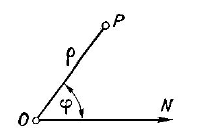
\includegraphics[width=0.25\textwidth]{la.png}
\end{wrapfigure}
$ON$ -- полярная ось. $\rho$ -- расстояние до точки $P$. $\varphi$ -- угол между осью и радиус-вектором из начала координат до точки $P$.
\newline
\newline
$(x,y)\,\Leftrightarrow\,(\varphi,\rho);$
\newline
\newline 
$x=\rho\cdot\cos\varphi,\,y=\rho\cdot\sin\varphi;\:\:\rho\sqrt{x^2+y^2},\,\tan\varphi=\frac{y}{x}$.


$z=\rho\cdot(\cos\varphi+i\cdot\sin\varphi)$ -- \textbf{тригонометрическая форма} записи к.ч., где $\varphi=arg\,z$ -- аргумент к.ч. (с точностью до $2\pi$).
\newline
\newline
$e^{i\varphi}=\cos\varphi+i\cdot\sin\varphi$ -- формула Эйлера. Тогда $z=\rho\cdot e^{i\varphi}$ -- \textbf{показательная форма} записи к.ч.
\newpage
\textbf{НОРМИРОВАННАЯ АЛГЕБРА КОМПЛЕКСНЫХ ЧИСЕЛ}
\newline
\newline
Пусть определена операция умножения для комплексных чисел так, чтобы выполнялись следующие условия:
\begin{enumerate}
    \item $|z_1\cdot z_2|\leqslant|z_1|\cdot|z_2|$
    \item Выполнялись аксиомы 9 и 10 для алшебры:
    \begin{enumerate}
        \item $\alpha\cdot(z_1\cdot z_2)=(\alpha\cdot z_1)\cdot z_2=z_1\cdot(\alpha\cdot z_2)$
        \item $(z_1+z_2)\cdot z_3=z_1\cdot z_3+z_2\cdot z_3$
    \end{enumerate}
\end{enumerate}
Получим нормированную алгебру с единицей $e=(1,0)$.
\newline
\newline
Положим $z_1=x_1+iy_1,\,z_2=x_2+iy_2$ и $i^2=-1$. Тогда:
\newline 
$z_1\cdot z_2=(x_1\cdot x_2-y_1\cdot y_2)+i(x_1\cdot y_2+x_2\cdot y_1)$ -- алгебраическая форма произведения. 
\newline 
$z_1\cdot z_2=(x_1\cdot x_2-y_1\cdot y_2,\,x_1\cdot y_2+x_2\cdot y_1)$ -- декартовая форма. 
\newline $z_1\cdot z_2=r_1\cdot r_2(\cos(\varphi_1+\varphi_2)+i\cdot\sin(\varphi_1+\varphi_2))$ -- тригонометрическая форма. 
\newline 
$z_1\cdot z_2=r_1\cdot r_2\cdot e^{i(\varphi_1+\varphi_2)}$ -- показательная форма.
\newline
\newline

\begin{wrapfigure}{r}{0.3\textwidth}
    \centering
    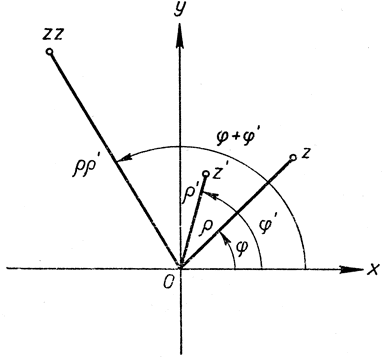
\includegraphics[width=0.25\textwidth]{ko.png}
\end{wrapfigure}
\textbf{Геометрический смысл} произведения $z\cdot z'$.
\newline
\newline
$z=|z|\cdot(\cos\varphi+i\sin\varphi),\,z'=|z'|\cdot(\cos\varphi'+i\sin\varphi')$
\newline
\newline
$z\cdot z'=|z|\cdot|z'|\cdot(\cos(\varphi+\varphi')+i\sin(\varphi+\varphi'))$
\newline
\newline
Умножение = поворот + растяжение ($|z'|>1$) или сжатие ($|z'|<1$).

\newpage
\section{Операция сопряжения и деления на множестве комплексных чисел, основные свойства. Поле комплексных чисел. Свойства экспоненты чисто мнимого числа. Формулы Эйлера, Муавра, корня n – ой степени. Вычисление квадратного корня в алгебраическом виде. Примеры.}
Назовём \textbf{сопряжённым} к числу $z=x+iy$ число $\overline{z}=x-iy$. В показательной записи: $z=r\cdot e^{i\varphi},\,\overline{z}=r\cdot e^{-i\varphi}$.
\n 
\textbf{Свойства:}
\begin{enumerate}
    \item $\overline{\overline{z}}=z$
    \item $\overline{z}=z\,\Leftrightarrow\,z\in\R$
    \item $\overline{z_1+z_2}=\overline{z_1}+\overline{z_2}$
    \item $\overline{z_1\cdot z_2}=\overline{z_1}\cdot\overline{z_2}$
    \item $Re\, z=\frac{z+\overline{z}}{2}$
    \item $Im\,z=\frac{z-\overline{z}}{2i}$
    \item $z\cdot\overline{z}=|z|^2$
    \item $\forall\,z\neq 0\::\:z^{-1}=\frac{\overline{z}}{|z|^2}$, $z\cdot z^{-1}=e=1$
\end{enumerate}
Из свойства 8 следует, что $\mathbb{C}$ -- поле.
\newline
\newline
\textbf{Частным} двух комплексных чисел $z_1$ и $z_2$ называют такое $z$, что
$$z=\frac{z_1}{z_2}=\frac{x_1\cdot x_2+y_1\cdot y_2}{x_2^2+y_2^2}+i\cdot\frac{x_2\cdot y_1-x_1\cdot y_2}{x_2^2+y_2^2} = \frac{|z_1|}{|z_2|}\cdot(\cos(\varphi_1-\varphi_2)+i\cdot\sin(\varphi_1-\varphi_2)) = \frac{r_1}{r_2} \cdot e^{i(\varphi_1 - \varphi_2)} $$

Из этого получаем ещё одно свойство сопряжения:
$$ \overline{\left(\frac{z_1}{z_2}\right)}=\frac{\overline{z_1}}{\overline{z_2}} $$
\newpage
\subsection{Формулы Эйлера, формула Муавра, корень $n$-ой степени}
\subsubsection{Формулы преобразований}
\begin{enumerate}
    \item $\forall\,k\in\Z:\;e^{i2\pi k}=1$
    \item $e^{i\varphi_1}\cdot e^{i\varphi_2}=e^{i(\varphi_1+\varphi_2)}$
    \item $e^{i(\varphi+2\pi k)}=e^{i\varphi}\:\forall\,k\in\Z$
    \item $|e^{i\varphi}|=1$
    \item $e^{-i\varphi}=\frac{1}{e^{i\varphi}}\::\:e^{-i\varphi}=\overline{e^{i\varphi}}$
\end{enumerate}
\subsubsection{Формулы Эйлера}
    \begin{enumerate}
        \item $\cos\varphi=\cfrac{e^{\varphi}+e^{-i\varphi}}{2}$
        \item $\sin\varphi=\cfrac{e^{\varphi}-e^{-i\varphi}}{2i}$
    \end{enumerate}
\subsubsection{Формула Муавра}
    
    $$z = (\cos(\varphi) + i\sin(\varphi)) \; \Rightarrow \; z^n=r^n\cdot(\cos(n\varphi)+i\sin(n\varphi))$$
    
\subsubsection{Извлечение корня $n$-ой степени}
    
    $$\sqrt[n]{z}=\sqrt[n]{r}\cdot\left(\cos\left(\frac{\varphi+2\pi k}{n}\right)+i\cdot \sin\left(\frac{\varphi+2\pi k}{n}\right)\right)$$
    
    Таким образом, у любого комплексного числа есть $n$ различных корней $n$-ой степени, так как в формулу можно подставить только $n$ различных $k$, потому как для $k_1 \equiv k_2 \mod (n)$ верно:
    \begin{equation*}
    	\begin{aligned}[t]
    		\cos\left(\frac{\varphi+2\pi k_1}{n}\right) = \cos\left(\frac{\varphi+2\pi k_2}{n}\right) \\
    		\sin\left(\frac{\varphi+2\pi k_2}{n}\right) = \sin\left(\frac{\varphi+2\pi k_2}{n}\right)
    	\end{aligned}
    \end{equation*}

\newpage
\section{Функции комплексного аргумента}
\subsection{Экспонента}
$$ exp(z)=e^{x+iy}=e^x\cdot e^{iy}=e^x(\cos y+i\sin y) = |z| \cdot e^{i \arg z} $$

\subsection{Логарифм}
$$ \ln\,z=\ln(|z|e^{i \arg z})=\ln|z|+i\arg z+2\pi i k $$

\subsection{Возведение в комплексную степень комплексного числа}
$$ (x_1+iy_1)^{x_2+iy_2}=e^{(x_2+iy_2)\ln(x_1+iy_1)}=e^{(x_2+y_2)\big(\ln\sqrt{x_1^2+i y_1^2}+i(\arctan\frac{y_1}{x_1}+2\pi n)\big)},\,n\in\Z$$

\subsection{Тригонометрические функции}
Для определения тригонометрических функций от комплексного аргумента сначала определим несколько вспомогательных функций:

\subsubsection{Гиперболический синус:}
	$$\sh x = \frac{e^x - e^{-x}}{2}$$
	
\subsubsection{Гиперболический косинус:}
	$$\ch x = \frac{{e^x} + e^{-x}}{2}$$

\subsubsection{Гиперболический тангенс:}
	$$\th x = \frac{\sh x}{\ch x} = \frac{e^x - e^{-x}}{e^x + e^{-x}}$$
	
\subsubsection{Свойства гиперболических функций:}
	\begin{enumerate}
		\item $\ch^2x - \sh^2x = 1$
		\item $\sh x = -i\sin(ix)$
		\item $\ch x = \cos(ix)$
		\item $\th x = -i\tg(ix)$
	\end{enumerate}
Стоит упомянуть, что гиперболический синус в устной речи называют \textit{шинусом}, а гиперболический косинус "--- \textit{чосинусом}.

\subsubsection{Тригонометрические функции комплексного аргумента:}

$\sphericalangle \: (a + bi) = z \in \mathbb{C}$, тогда:
\begin{itemize}
	\item $\sin z = \sin a \cos (bi) + \cos a \sin (bi) = \sin a \ch b + i\cos a \sh b$
	\item $\cos z = \cos a \cos (bi) + \sin a \sin (bi) = \cos a \ch b - i\sin a \sh b$
\end{itemize}


Помимо этого, можно просто пользоваться выражением тригонометрических функций комплексного аргумента при помощи формулы Эйлера:

\begin{itemize}
	\item $\sin z = \frac{e^{iz} - e^{-iz}}{2i}$
	\item $\cos z = \frac{e^{ix} + e^{-iz}}{2}$
\end{itemize}

\subsection{Обратные тригонометрические функции:}

Для нахождения множества значений обратной тригонометрической функции от комплексного аргумента надо решать уравнение. Решим такие уравнения для обратных синуса и косинуса комплексного аргумента:

\begin{equation*}
	\begin{aligned}
		\arccos z = v, \; \Rightarrow \cos(\arccos z) = \cos v, \; \Rightarrow z = \cos v = \frac{e^{iv} + e^{-iv}}{2},\; \Rightarrow e^{2iv} - e^{iv} \cdot (2z) + 1 = 0,\;\Rightarrow\\
		\Rightarrow e^{iv} = \frac{2z + \sqrt{4z^2 - 4}}{2} = z + \sqrt{z^2 - 1},\;\Rightarrow v = -i \cdot \ln \left(z + \sqrt{z^2 - 1}\right) =\\
		= -i \cdot \left(\ln |z + \sqrt{z^2 - 1}| + i \arg (z + \sqrt{z^2 - 1}) + 2\pi i k\right)
	\end{aligned}	
\end{equation*}

\begin{equation*}
	\begin{aligned}
		\arcsin z = v, \; \Rightarrow \sin(\arcsin z) = \sin v, \; \Rightarrow z = \sin v = \frac{e^{iv} - e^{-iv}}{2i},\; \Rightarrow e^{2iv} - e^{iv} \cdot (2iz) - 1 = 0,\;\Rightarrow\\
		\Rightarrow e^{iv} = \frac{2iz + \sqrt{4 - 4z^2}}{2} = iz + \sqrt{1 - z^2},\;\Rightarrow v = -i \cdot \ln \left(iz + \sqrt{1 - z^2}\right) =\\
		= -i \cdot \left(\ln |iz + \sqrt{1 - z^2}| + i \arg (iz + \sqrt{1 - z^2}) + 2\pi i k\right)
	\end{aligned}
\end{equation*}

\newpage
\section{Линейная оболочка, линейная независимость векторов. Теорема о линейно независимых системах векторов,
следствие. Теорема о «прополке».}
$V$ -- линейное (векторное пространство) над полем $K$. Если $K=\R$, то $V$ -- вещественное
(действительное) линейное пространство, если $K=\mathbb{C}$, то $V$ -- комплексное линейное
пространство.

\subsection{Определения}
Вектор $u\in V$ называется линейной комбинацией векторов $v_1,\ldots,v_m$, если существуют такие скаляры $\lambda_1,\ldots,\lambda_m\in K$, что $u=\lambda_1v_1+\ldots+\lambda_m v_m$.

Линейной оболочкой векторов $v_1,\ldots,v_m$ называется множество их всевозможных линейных комбинаций.
$$ span(v_1,\ldots,v_m)=\{\lambda_1v_1+\ldots+\lambda_m v_m\,|\,\lambda_i\in K\} $$

Система векторов $v_1,\ldots,v_m$ называется линейно независимой, если их линейная комбинация $u=\lambda_1v_1+\ldots+\lambda_m v_m$ равна нулю тогда и только тогда, когда $\lambda_1=\ldots=\lambda_m=0$. В противном случае система называется линейно зависимой.

\subsection{Теорема о линейно независимых системах векторов}
\subsubsection{Ну сама теорема}
\begin{enumerate}
    \item Система векторов линейно зависима тогда и только тогда, когда один из векторов системы является линейной комбинацией остальных.
    \item Если некоторая подсистема системы векторов линейно зависима, то линейно зависима вся система.
    \item $v_1,\ldots,v_m$ -- линейно независимая система. Если $v_1,\ldots,v_m,v_{m+1}$ линейно зависима, то $v_{m+1}$ -- линейная комбинация $v_1,\ldots,v_m$.
\end{enumerate}

\textbf{Доказательство}
\begin{enumerate}
    \item Перая часть
    \begin{enumerate}
        \item \textit{Система векторов линейно зависима тогда и только тогда, когда один из векторов системы является линейной комбинацией остальных.}
        
        Существуют такие скаляры $\lambda_1,\ldots,\lambda_m\in K$ не все нули, $\lambda_1v_1+\ldots+\lambda_m v_m=0$. Перенесём $\lambda_m v_m$ в правую сторону и поделим на $-\lambda_m$, получимм $v_m=\cfrac{\lambda_1v_1+\ldots+\lambda{m-1} v_{m-1}}{-\lambda_m}$, то есть $v_m$ -- линейная комбинация остальных векторов.
        \item \textit{Один из векторов системы является линейной комбинацией остальных тогда и только тогда, когда система векторов линейно зависима.}
        
        Скаляры $\lambda_1,\ldots,\lambda_m\in K$ не все нули. Линейная комбинация $v_m=\lambda_1v_1+\ldots+\lambda{m-1} v_{m-1}\,\Leftrightarrow\,\lambda_1v_1+\ldots+\lambda{m-1} v_{m-1}-v_m=0$ -- это и есть линейно зависимая система векторов по определению.
    \end{enumerate}
    \item Система векторов $v_1,\ldots, v_m$. Пусть $v_1,\ldots,v_k$ -- линейно зависимая система, $k<m$. Тогда существуют $\lambda_1,\ldots,\lambda_k$ не все нули, что линейная комбинация $\lambda_1v_1+\ldots+\lambda_k v_k=0$. Допустим, выразим вектор $v_k$ как линейную комбинацию остальных, тогда исходная система $v_1,\ldots,v_m$ тоже будет содержать этот вектор, линейно зависимый от предыдущих, значит, сама система тоже будет являться линейно зависимой.
    \item Скаляры $\lambda_1,\ldots,\lambda_m,\lambda_{m+1}$ не все нули, линейная комбинация $\lambda_1v_1+\ldots+\lambda_m v_m+\lambda v_{m+1}v_{m+1}=0$. Выражаем $v_{m+1}=\cfrac{\lambda_1v_1+\ldots+\lambda_m v_m}{-\lambda_{m+1}}$, вуаля
\end{enumerate}
\subsubsection{Следствия}
\begin{enumerate}
    \item Система векторов линейно независима тогда и только тогда, когда любая её подсистема линейно независима.
    \item Любая система, содержащая нулевой вектор, линейно зависима.
    \item Любая система, содержащая два пропорциональных вектора (в частности, два равных), линейно зависима.
\end{enumerate}

\subsection{Теорема о прополке!!!}
Если система векторов $v_1,\ldots,v_n$ содержит хотя бы один ненулевой вектор, то из неё можно выделить линейно независимую подсистему таким образом, что линейная оболочка не изменится.

\textbf{Доказательство}
$$ s_0=span(0) $$
$$ s_1=span(v_1) $$
$$\ldots$$
$$ s_n=span(v_1,\ldots,v_n) $$
Наше подмножество подразумевает, что $s_0\subseteq s_1\subseteq \ldots \subseteq s_{n-1}\subseteq s_n$. Если $s_n=s_{n-1}$, то уберем вектор $v_n$ из набора. Тогда $v_m\in s_m \land \in s_{m-1} \,\Rightarrow\,v_m$ -- линейная комбинация $v_1,\ldots,v_{n-1}$. Повторяем эти действия, пока не дойдем до $s_0$ и $s_1$. Таким образом совершили прополку, остались $s_0\subset s_1\subset\ldots\subset s_k$, где оставшиеся $k$ векторов -- линейно независимая система. Доказали.

\newpage
\section{Порождающая система векторов, конечномерные пространства. Теорема об эквивалентных условиях для базиса. Размерность пространства. Теорема о дополнении любой независимой системы до базиса и о порождающей системе векторов.}
\subsection{Порождающая система векторов, конечномерные пространства}
Совокупность векторов называется \textbf{порождающей} (полной), если все элементы пространства $V$ являются линейной комбинацией этих векторов.

Линейное пространство называется \textbf{конечномерным}, если в нем существует конечная порождающая система, иначе пространство называется \textbf{бесконечномерным}.

\subsection{Теорема об эквивалентных условиях для базиса}
Следующие утверждения эквивалентны
\begin{enumerate}
    \item $v_1,\ldots,v_n$ -- порождающий и линейно независимый.
    \item $v_1,\ldots,v_n$ -- максимальный по числу элементов линейно неазвисимый набор.
    \item $v_1,\ldots,v_n$ -- минимальный по числу элементов порождающий набор.
\end{enumerate}

\textbf{Доказательство}
\begin{enumerate}
    \item $1\to2$
    
    Предположим, что набор $v_1,\ldots,v_n$ не максимальный (по числу элементов) линейно независимый набор. Тогда можно добавить еще один вектор $v_{n+1}$ так, что система векторов останется линейно независимой. Однако, он выражается через набор $v_1,\ldots,v_n$, так как этот набор порождающий. Следовательно,$v_1,\ldots,v_{n+1}$ -- линейно зависимый набор векторов, а тогда наше предположение неверно, и $v_1,\ldots,v_n$ - максимальный набор.
    \item $2\to1$
    
    $v_1,\ldots,v_n$ -- максимальный набор линейно независимых векторов, а тогда для любого вектора $u\in V$ верно, что $u,v_1,\ldots,v_n$ -- линейно зависимый набор, а тогда $u$ -- линейная комбинация векторов $v_1,\ldots,v_n$, а значит, $v_1,\ldots,v_n$ -- порождающая система.
    \item $1\to3$
    
    
    \item $3\to1$
    
    Если $v_1,\ldots,v_n$ -- минимальный порождающий, но, предположим, что он линейно зависимый, значит какой-то вектор выражается через остальные, следовательно, если мы уберем его, то линейная оболочка не изменится. Тогда $v_1,\ldots,v_{n-1}$ тоже порождающий. Но это противоречит тому, что $v_1,\ldots,v_n$ -- минимальный порождающий. Значит, наше предположение неверно и $v_1,\ldots,v_n$ -- линейно независимый.
\end{enumerate}
\subsection{Размерность пространства}
Совокупность векторов, удовлетворяющих условиям \textit{Теоремы об эквивалентных условия} называется \textbf{базисом}. Число элементов базиса $n=dim(V)$ называется \textbf{размерностью} пространства $V$.
\subsection{Теорема о дополнении любой независимой системы до базиса и о порождающей системе векторов}
\begin{enumerate}
    \item Любая линейно независимая система может быть дополнена до базиса.
    \item Любая порождающая система содержит базис.
\end{enumerate}

\textbf{Доказательство}

\begin{enumerate}
    \item Если линейно независимая система максимальная по числу элементов, то она уже является базисом. Если нет, то... если система векторов $v_1,\ldots,v_n$ -- линейно независимая система, то мы можем добавить в неё какой-то вектор $v_{m+1}$, сохраняя при этом линейную независимость системы. Делаем так, пока не наберем максимальное количество элементов и не получим базис.
    \item Если система минимальная по количеству элементов порождающая, то это базис. Если не минимальная, то среди векторов найдется вектор, являющийся линейной комбинацией остальных. Этот вектор можно убрать. Делаем это, пока не получим минимальную по количествам элементов порождающую систему -- то есть базис.
\end{enumerate}

\newpage
\section{Координаты вектора и их единственность. Изоморфизм линейных пространств и его свойства. Теорема об изоморфизме конечномерных пространств, следствия.}
\subsection{Координаты вектора и их единственность}
Пусть $V$ -- линейное пространство ($dim\,V=n$), а $\overline{e}_1,\ldots,\overline{e}_n$ -- его базис. Тогда любой вектор $\overline{x}$ можно представить в виде $\overline{x}=x_1\overline{e}_1+\ldots+x_n\overline{e}_n$, где $x_1,\ldots,x_n$ -- \textbf{координаты} вектора $\overline{x}$.

\textbf{Утверждение.} Координаты вектора определяются единственным образом.

\textbf{Доказательство}

Пусть вектор $\overline{x}$ имеет координаты $x_1,\ldots,x_n$ и координаты $x_1',\ldots,x_n'$ (всё в том же пространстве и том же базисе). Тогда $\overline{x}=\sum x_i\overline{e}_i=\sum x_i'\overline{e}_i$. То есть, $\sum(x_i-x_i')\overline{e}_i=0\,\Leftrightarrow\,x_i-x_i'=0$. Следовательно, все координаты $x_i$ равны соответственно координатам $x_i'$, что и требовалось доказать.

\subsection{Изоморфизм и прелести}
\subsubsection{Определение}
\textbf{Изоморфизмом} называется взаимо-однозначное соответствие между линейными пространствами. Линейные пространства, имеющие взаимо-однозначное сооветствие, называются изоморфными.

Допусти $V_1$ и $V_2$ -- линейные пространства над полем $K$. Они называются \textbf{изоморфными}, если между их элементами существует взаимооднозначное соответствие, то есть:

$$ f\::\:V_1\to V_2 $$
$$ \forall\,v_1,v_2\in V_1\::\:f(v_1+\lambda\cdot v_2)=f(v_1)+\lambda\cdot f(v_2) \in V_2$$

\subsubsection{Свойства}
\begin{enumerate}
    \item Нулевые элементы изоморфных ЛП соответствуют друг другу.
    \item Противоположные элементы соответствуют друг другу.
    \item Линейной комбинации векторов пространства $V_1$ соответствует линейная комбинация соответствующих векторов пространства $V_2$.
    \item Если пространство $V_1$ изоморфно пространству $V_2$, а $V_2$ изоморфно пространству $V_3$, то пространства $V_1$ и $V_3$ также изоморфны.
    \item Линейно независимой (линейно зависимой) (порождающей) системе векторов пространства $V_1$ соответствует линейно независимая (линейно зависимая) (порождающая) система векторов пространства $V_2$ (следствие из предыдущих свойств).
\end{enumerate}
\subsubsection{Теорема об изоморфизме конечномерных пространств}
\begin{enumerate}
    \item Если линейное пространство $V_1$ изоморфно конечномерному пространству $V_2$, то $V_1$ тоже является конечномерным пространством той же размерности.
    \item Если $V_1$ и $V_2$ -- линейные конечномерные пространства одной размерности, то они изоморфны.
\end{enumerate}

\textbf{Доказательство}

\begin{enumerate}
    \item $V_2$ изоморфно пространству $V_1$, следовательно, базис $V_1$ изоморфен базису $V_2$, то есть размерности их равны, ну логично дофига
    \item $e_1,\ldots,e_n$ -- базис $V_1$, $dim\,V_1=n=dim\,V_2$, $e_1',\ldots,e_n'$ -- базис $V_2$. Т.к. их размерности равны $n$, можно смело утверждать, что $V_1\leftrightarrow \R^n (\mathbb{C}^n)$ и $V_2\leftrightarrow \R^n(\mathbb{C}^n)$. А по следствию из свойства изоморфных линейных пространств, можно утверждать, что $V_1$ и $V_2$ -- изоморфны.
\end{enumerate}
\textbf{Следствия}
\begin{enumerate}
    \item Любое конечномерное пространство над полем $\R(\mathbb{C})$ размерности $n$ изоморфно $n$-мерному арифметическому пространству $\R(\mathbb{C}^n)$.
    \item Изоморфизм -- отношение эквивалентности на пространстве конечномерных линейных пространств.
\end{enumerate}

\newpage
\section{Теорема о линейном подпространстве. Примеры. База, ранг системы векторов. Теорема о ранге. Пересечение и сумма линейных подпространств. Формула Грассмана.}
\subsection{Определение ЛПП}
$L\subset V$ называется линейным подпространством $V$, если выполнены 1-8 аксиомы линейного пространства (то есть, $L$ -- тоже линейное пространство по отношению к определенным в $V$ операциям сложения векторов и умножения вектора на число).

\subsection{Теорема о линейном подпространстве}
\begin{enumerate}
    \item Если векторы $v$ и $u$ содержатся в $L$, то в $L$ содержатся и вектор $u+v$.
    \item Если вектор $u$ содержится в $L$, то в $L$ содержится и вектор $\lambda$ для всех $\lambda\in K$.
\end{enumerate}
То есть $L$ является ЛПП тогда и только тогда, когда оно замкнуто относительно $+$ и $\cdot\lambda$.

\textbf{Доказательство}

Необходимость следует из определения ЛПП.

Для доказательства достаточности, покажем лишь что выполняются 3 и 4 аксиомы (существование нуевого и противоположного элемента).
\begin{enumerate}
    \setcounter{enumi}{2}
    \item $\lambda=0$, возьмём элемент $\lambda\cdot v=0\cdot v=0$. Так как $\lambda\cdot v\in L,\Rightarrow\,0\in L$.
    \item $\lambda=-1$, возьмём элемент $\lambda\cdot v=(-1)\cdot v=0$. Так как $\lambda\cdot v\in L,\Rightarrow\,-v\in L$. Сумма $v+(-v)=0\in L$.
\end{enumerate}
\subsection{База}
$v_1,\ldots,v_n$ -- система векторов из $V$. Линейно независимый набор векторов $v_1,\ldots,v_k$ называется \textbf{базой} ($k<=m$), если линейные оболочки их и $v_1,\ldots,v_n$ совпадают, то есть $span(v_1,\ldots,v_n)=span(v_1,\ldots,v_k)$.
\subsection{Ранг}
\subsubsection{Определение}
\textbf{Рангом} системы векторов $v_1,\ldots,v_n$ называется размерность его линейной оболочки $span(v_q,\ldots,v_n)$, то есть $rg(v_1,\ldots,v_n)=dim(span(v_1,\ldots,v_n))$.

\newpage
\subsubsection{Элементарные преобразования системы векторов}
\begin{enumerate}
    \item Добавление (удаление) нулевого вектора.
    \item Умножение некоторого вектора набора на скаляр $\lambda\in K$.
    \item Перестановка двух векторов набора местами.
    \item Замена некоторого вектора на его сумму с другим.
\end{enumerate}
\subsubsection{Теорема о ранге}
Линейная оболочка системы векторов не меняется при элементарных преобразованиях.

\textbf{Доказательство}

1 - 3 очевидны из определения линейной оболочки.

Чтобы доказать 4 пункт, нужно доказать, что линейные оболочки, натянутые на наборы векторов $v_1,\ldots,v_i,\ldots,v_j,\ldots,v_n$ и $v_1,\ldots,v_i,\ldots,v_j+v_i,\ldots,v_n$, совпадают, то есть любой вектор из одной оболочки принадлежит другой оболочке, и наоборот.

Путсь вектор $\lambda_1 v_1+\ldots+\lambda_i v_i+\ldots+\lambda_j v_j+\ldots+\lambda_n v_n$ принадлежит оболочке первой системы векторов, тогда тот же вектор, записанный в виде $\lambda_1 v_1+\ldots+(\lambda_i+\lambda_j-\lambda_j)v_i+\ldots+\lambda_j v_j+\ldots+\lambda_n v_n=\lambda_1 v_1+\ldots+(\lambda_i-\lambda_j)v_i+\ldots+\lambda_j(v_j+v_i)+\ldots+\lambda_n v_n$ так же принадлежит и оболочке второй системы векторов, обратное доказательство то же самое. Раз линейная оболочка не меняется, то не меняется её размерность, а следовательно и ранг.

\subsection{Пересечение и сумма ЛПП}
\subsubsection{Определения}
\textbf{Пересечением} ЛПП $L_1$ и  $L_2$ называется множество $L_1\cap L_2$ векторов, каждый из которых принадлежит и $L_1$, и $L_2$. 

\textbf{Суммой} ЛПП $L_1$ и $L_2$ называется множество $L_1+L_2$ векторов, каждый из которых представляется в виде $v+u$, где $v\in L_1,\,u\in L_2$.

\subsubsection{Формула Грассмана}
$$ dim(L_1\cap L_2)=dim\,L_1+dim\,L_2-dim(L_1+L_2)$$
\textbf{Доказательство}

МНЕ ПОКА ЛЕНЬ Я ПРОПУЩУ

\href{http://mathhelpplanet.com/static.php?p=peresechenie-i-summa-podprostranstv}{Доказательство}

\newpage
\section{Прямая сумма линейных подпространств. Теорема об эквивалентных условиях прямой суммы, следствие. Проекции вектора на линейные подпространства. Примеры. Теорема о совпадении линейных многообразий, следствие. Примеры.}
\subsection{Прямая сумма}
\subsubsection{Определения}
Линейные подпространства $L_1,\ldots,L_n$ называются дизъюнктными, если $\forall x_i\in L_i, \,i=1,\ldots,n\::\:x_1+\ldots+x_n=0\,\Leftrightarrow\,x_i=0$ -- действует единственность разложение нулевого вектора.

Тогда, сумма линейных подпространств $L_1,\ldots,L_n$ называется прямой суммой $L_1\oplus\ldots\oplus L_n$, если линейные подпространства $L_1,\ldots,L_n$ дизъюнктны.

\subsubsection{Теорема об эквивалентных условиях прямой суммы}
Сумма является прямой тогда и только тогда, когда 
\begin{enumerate}
    \item $L=\sum\limits_{i=1}^n L_i$  и $L_j\cap(\sum\limits_{\substack{i=1\\i\neq j}}^n L_i)=0$
    \item $\forall\,x\in L\::\:x=x_1+\ldots+x_n$ -- представление однозначно через $x_i\in L_i$
    \item Объединение базисов $L_1,\ldots,L_n$ равно базису $L$.
\end{enumerate}
\textbf{Доказательство}

\begin{enumerate}
    \item $(\Rightarrow)$
    
    По условию, $L_1,\ldots,L_n$ -- дизъюнктны. Рассмотрим $x\in L_j\cap (\sum L_i)\,\Leftrightarrow\,(x\in L_j)\land (x\in \sum L_i),\,i=1\ldots n,i\neq j$, то есть $x=x_j=x_1+\ldots+x_n,\,i=1\ldots n,\,i\neq j$. Перенесём $x_j$ в правую часть, получим $x_1+\ldots+x_n-x_j=0$. Т.к. все $L_i$ дизъюнктные, то получаем, что $x_i=0\,,i=1\ldots n$. Значит, $x$ тоже равен нулю. А раз $x\in L_j\cap (\sum L_i)$ и $x=0$, то следует, что $L_j\cap \sum L_i),\,i=1\ldots n,i\neq j=0$, что и требовалось доказать.
    
    $(\Leftarrow)$
    
    $L_j\cap \sum L_i=0,\,i=1\ldots n,i\neq j=0$. Возьмём любую комбинацию элементов $x_i\in L_i$ и выразим из неё $x_j$: $x_j=-x_1-\ldots-x_n$. Тогда получаем, что $x_j\in L_j\cap (\sum L_i),\,i=1\ldots n,\,i\neq j$ (очему-то, я реально не понимаю почему). В принципе, тогда значит, что $x_j=0\,,j=1\ldots n$, то есть нулевой элемент представляется единсвенным образом при всех $x_i=0$ в комбинации соответствующей (ну понятно). То есть $L_1,\ldots,L_n$ -- дизъюнктны.
    \newpage
    \item $(\Rightarrow)$
    
    Предположим обратно, что представление векторов через другие не однозначное, то есть
    $\begin{cases} x=x_1+\ldots+x_n\\x=x_1'+\ldots+x_n' \end{cases}$
    
    Вычтем из первого уравнения второе, получим $0=(x_1-x_1')+\ldots+(x_n-x_n')$. Скобки $(x_1-x_1')\in L_1,\ldots,(x_n-x_n')\in L_n$. Так как сумма прямая, то получаем, что $x_i-x_i'=0,\,i=1\ldots n$ \textit{(из первого условия что ли? про разложение нулевого вектора)}, значит $x_i=x_i'$, то есть разложение однозначно.
    
    $(\Leftarrow)$
    
    Дано, что разложение любого элемента однозначно, то есть $x=x_1+\ldots+x_n,\,x_i\in L_i$. Ну предположим, что существует какой-то $x'\neq 0,\,x'\in L_1\cap L_2$ (необязательно 1 и 2, любых хотя бы двух ЛПП). Тогда элемент $x$ можно представить как $x=(x_1+x')+(x_2-x')+\ldots+x_n$, то есть разложение не единственно! Противоречит условию, верно обратное.
    
    \item $(\Rightarrow)$
    
    Для простоты возьмём только два ЛПП $L$ и $M$. Базис $L$ равен $(e_1,\ldots,e_n$, базис $M$ равен $t_1,\ldots,t_k$. Возьмём произвольный элемент $x$, тогда из определеняи прямой суммы (однозначное представление любого элемента $L$) следует, что существует единственная пара векторов $(l,m)$ такая, что $x=l+m$. Разложим вектора $l$ и $m$ по базисам $L$ и $M$ соответственно: $l=l_1e_1+\ldots+l_n e_n$ и $m=m_1t_1+\ldots+m_k t_k$. Так как вектора по базисам свои раскладываются однозначно, то и вектор $x$ представляется в сумме базисов $(e_1\ldots,e_n)$ и $(t_1,\ldots,t_k)$ тоже однозначно.
    
    $(\Leftarrow)$
    
    Возьмем два ЛПП $L$ и $M$. Базис $L$ равен $(e_1,\ldots,e_n$, базис $M$ равен $t_1,\ldots,t_k$, их объединение \textit{пока оставлю}
\end{enumerate}
\textbf{Следствие}

$$L=L_1\oplus \ldots\oplus L_n\,\Rightarrow\,dim\,L=\sum dim\,L_i$$
\subsection{Проекции вектора на ЛПП}
Пусть $L+L_1\oplus\ldots\oplus L_n$ и $\forall\,x\in L$ представляется однозначно $x=x_1+\ldots+x_n$, где $x_i\in L_i$ -- \textbf{проекция} элемента $x$ на ЛПП $L_i$ параллельно остальным ЛПП.

\textbf{Утверждение}

Базис подпространства $L\subset V$ всегда можно дополнить до базиса линейного пространства $V$.

Пример -- $\overline{k}$ и $\overline{i},\,\overline{j}$ образуют в пространстве прямую сумму -- прсотранство векторов.
\newpage
\subsection{Линейные многообразия}
\subsubsection{Определение}
\textbf{Линейным многообразием} назывется множество $P=x_0+L=\{x+0+l\,|\,l\in L\}$, где $L$ -- линейное подпространство $V$ и $x_0\in V$

\subsubsection{Теорема о совпадении линейных многообразий}

Пусть $L_1,\,L_2\in V;\;x_1,\,x_2\in V$ и пусть есть многообразтия $P_1=x_1+l,\,P_2=x_2+L_2$, тогда
$$ P_1=P_2\,\Leftrightarrow\,L_1=L_2=L;\;(x_1-x_2)\in L $$
\textbf{Доказательство}

($\Rightarrow$)

Пусть $P_1=P_2$, тогда $x_1+l_1=x_2+l_2\,\Rightarrow\,x_1-x_2+l_1=l_2$. Пусть $l_1=0\::\:x_1-x_2=l_2\in L_2$. Пусть $l_1=x_2-x_1+l2$, а так как $x_2-x_1\in L_2$, то любой $l_1\in L_2,\,l_1\in L_1$, аналогично для $l_2$. Следовательно, $L_1=L_2=L$, ч.т.д.

($\Leftarrow$)

Преобразуем $x_1=x_1$ как $x_1+l=x_1-x_2+x_2+l$. По условию $x_1-x_2\in L=L_2;\;l\in L= L_2$, тогда примем $x_1-x_2+l=l_2\in L_2$, тогда $x_1+l=x_2+l_2\,\Rightarrow\,P_1=P_2$

\textbf{Следствие}

$$ P+x_0+L;\;x_1\in P\,\Rightarrow\,P_1=x_1+L;\;P_1=P $$

\newpage
\section{Матрицы: основные понятия. Основные алгебраические операции над матрицами и их свойства. Алгебра матриц.}

\subsection{Основные определения}
\textbf{Матрица} размерности $m \times n$ (записывается как $A_{m\times n}$) "--- таблица из $m$ строк и $n$ столбцов, заполненная некоторыми элементами $A_{i, j}$.

\textbf{Квадратная матрица} "--- матрица размера $n\times n$.

\textbf{Главная диагональ матрицы} (определена только для квадратных матриц) "--- такие элементы $A_{i, j}$, что $i = j$.

\textbf{Побочная диагональ матрицы} (определена только для квадратных матриц) "--- такие элементы $A_{i, j}$, что $i + j = n$.

\textbf{Согласованные матрицы} "--- пара матриц $A_{n\times m}$ и $B_{m 'times k}$.

\subsection{Алгебраические операции}
\subsubsection{Сложение}
\begin{enumerate}
    \item $A_{m\times n},\,B_{m\times n},\,\exists\, C_{m\times n}=A+B$
    \item $\forall\,i,j:\;c_{ij}=a_{ij}+b_{ij}$
    \item $A+\mathbb{O}=\mathbb{O}+A=A$
    \item Можно складывать матрица только одной размерности.
    \item Сложение коммутативно, ассоциативно, с нулевым элементом, с противоположным элементом.
\end{enumerate}
\subsubsection{Умножение на число}
\begin{enumerate}
    \item $A_{m\times n},\,\exists\,D_{m\times n}=\lambda\cdot A$
    \item $d_{ij}=\lambda\cdot a_{ij}$
    \item $\alpha\cdot(\beta\cdot A)=(\alpha\cdot\beta)\cdot A$
\end{enumerate}
\subsubsection{Вычитание}
	$A - B = A + (-1)\cdot B$, свойства из предыдущих двух пунктов.
\subsubsection{Произведение матриц}
\begin{enumerate}
    \item ($A$ и $B$ -- согласованные)$A_{m\times n},\,B_{n\times k},\,\exists C_{m\times k}=A\cdot B$
    \item $c_{ij}=\sum\limits_{k=1}^n a_{ik}\cdot b_{kj}$ (столбец на строку)
    \item Существует едтиничная матрица $\mathcal{I}\::\:A\cdot \mathcal{I} = \mathcal{I} \cdot A =A$
    \item Если определены $A\cdot B$ и $B\cdot A$, то $A$ и $B$ -- квадратные.
\end{enumerate}
\newpage
\subsection{Алгебра матриц}
\textbf{Свойства} $\forall\,A,B,C;\;\forall\,\alpha,\beta\in K$
\begin{enumerate}
    \item $A+B=B+A$
    \item $(A+B)+C=A+(B+C)$
    \item $\exists\,\mathbb{O}\::\:A+\mathbb{O}= \mathbb{O} + A = A$
    \item $\exists\, \mathcal{I}\::\:A\cdot \mathcal{I}=\mathcal{I} \cdot A = A$
    \item $\forall\,A\:\exists \,-A\::\:A+(-A)=\mathbb{O}$
    \item $\alpha\cdot(A+B)=\alpha\cdot A+\alpha\cdot B$
    \item $(\alpha+\beta)\cdot A=\alpha\cdot A+\beta\cdot A$
    \item $(\alpha\cdot\beta)\cdot A=\alpha\cdot(\beta\cdot A)=\beta\cdot(\alpha\cdot A)$
    
    Получаем линейное пространство матриц $M_{m\times n}$:
    $$ M_{m\times n}\cong\R^{m+n}\,(\mathbb{C}^{n+m}) $$
    \item $(A+B)\cdot C=A\cdot C+B\cdot C;\;A\cdot
    (B+C)=A\cdot B+A\cdot C$
    \item $\alpha\cdot(A\cdot B)=(\alpha\cdot A)\cdot B=A\cdot(\alpha\cdot B)$
    \item $(A\cdot B)\cdot C=A\cdot(B\cdot C)$
\end{enumerate}
(1) - (10) -- алгебра, (1) - (11) -- ассоциативная алгебра.
\newpage
\section{Операция транспонирования и её свойства. Обратная матрица и её свойства.}
\subsection{Операция транспонирования}
\subsubsection{Определение}
Транспонированной матрицы $A$ называют такую матрицу $A^T$, что для $\forall i, j:\; A^T_{i, j} = A_{j, i}$.
\subsubsection{Свойства}
\begin{enumerate}
    \item $(A^T)^T=A$
    \item $(A+B)^T=A^T+B^T$
    \item $(A\cdot B)^T=B^T\cdot A^T$
    \item $(\lambda\cdot A)^T=\lambda\cdot A^T$
    \item $\mathcal{I} = \mathcal{I}^T$
\end{enumerate}
Докажем третье свойство.

Пусть $A_{m\times n}$ и $B_{n\times k}$ -- согласованные. Тогда $B^T_{k\times n}$ и $A^T_{n\times m}$ -- тоже согласованные. Распишем:

$$ \begin{cases} ((A\cdot B)^T)_{ij}=(A\cdot B)_{ji}=\sum\limits_{r=1}^k a_{jr}\cdot b_{ri} \\ (B^T\cdot A^T)_{ij} = \sum\limits_{r=1}^k b_{ri}\cdot a_{jr} \end{cases} \Rightarrow\: (A\cdot B)^T = B^T\cdot A^T $$

\subsection{Обратная матрица}
\subsubsection{Определение}
Обратной матрицей для матрицы $A$ называют такую матрицу $A^{-1}$, что $A\cdot A^{-1} = \mathcal{I}$.
\subsubsection{Свойства}
\begin{enumerate}
    \item $A^{-1}$ -- единственна.
    
    \textbf{Доказательство:}
    
    Допустим, что существует еще одна обратная матрица $B$. Тогда
    $$\begin{cases} B\cdot A = \mathcal{I} \\ A^{-1}\cdot A = \mathcal{I} \end{cases}\Leftrightarrow\, \begin{cases} B\cdot A \cdot A^{-1} = \mathcal{I}\cdot A^{-1}=A^{-1} \\ B\cdot A\cdot A^{-1}=B\cdot \mathcal{I} = B \end{cases} \Rightarrow\: B=A^{-1}$$
    
    \item $(A^{-1})^{-1}=A$
    \item $(\lambda\cdot A)^{-1} = \cfrac{1}{\lambda}\cdot A^{-1}$
    \item $(A^T)^{-1}=(A^{-1})^T$
    \item $(A\cdot B)^{-1}=B^{-1}\cdot A^{-1}$
\end{enumerate}
\newpage
\section{Строчный и столбцовый ранги матрицы. Два утверждения и следствие о линейно независимых отрезках столбцов матрицы. Теорема о ранге матрицы.}

Дана матрица $A_{m\times n}$. Её можно записать как систему столбцов $(A_1,\ldots,A_n)$, либо как систему строк $(S_1,\ldots,S_m)^T$.

\textbf{Строчным рангом} $rg_{lin}$ матрицы $A$ называют размерность базиса линейной оболочки над системой векторов $(S_1,\ldots,S_m)$.

\textbf{Столбцовым рангом} $rg_{col}$ матрицы $A$ называют размерность базиса линейной оболочки над системой векторов $A_{m\times n}$.

\textbf{Отрезком} столбца/строки $S_i = (a_{1, i}, a_{2, i}, \ldots, a_{n, i})$ называют $\overline{S^k_i} = (a_{1, i}, a_{2, i}, \ldots, a_{k, i})$ю

\begin{comment}
	Рассмотрим систему столбцов $\overline{A_i}$, где $\overline{A_i}=(a_{1i},\ldots,a_{ki})^T$ -- отрезок столбца длины $k\leqslant n$ и $\overline{S_j}=(a_{j`},\ldots,a_{jk}$ -- отрезок строки фиксированной длины.
\end{comment}


\subsection{Вспомогательные утверждения}
\subsubsection{Утверждение 1}
Если $(A_1,\ldots,A_n)$ "--- линейно зависимая система векторов, то $\forall k \leq n:\:(\overline{A^k_1},\ldots,\overline{A^k_n})$ -- тоже линейно зависимая система векторов.

\textbf{Доказательство}

$(A_1,\ldots,A_n)$ "--- линейно зависимая система, следовательно, существует набор коэффициентов $\alpha_1,\ldots,\alpha_n:\: \sum\limits_{i = 0}^n \alpha_i^2 > 0$ такой, что $\sum\limits_{i=1}^n \alpha_i\cdot A_i = (0,\ldots,0)^T$ -- столбец из $m$ нулей. А так как первые $k$ элементов этого столбца тоже нули, то получаем, что $\sum\limits_{i=1}^k \alpha_i\cdot A_i=(0,\ldots,0)^T$ -- столбец из $k$ нулей, то есть $(\overline{A_1^k},\ldots,\overline{A^k_n})$ -- тоже линейно зависимы.

\textbf{Следствие из утверждения 1}

Если $\exists k:\: (\overline{A_1^k},\ldots,\overline{A^k_n})$ -- линейно независимы, то $(A_1,\ldots,A_n)$ -- тоже линейно независимы. Доказывается от обратного.

\subsubsection{Утверждение 2}
Если $rg_{lin} = r$ и $(S_1, S_2, \ldots S_k)$ "--- линейно независимая система, то, если $\exists k < r:\:(\overline{A^k_1}\ldots \overline{A^k_r})$ "--- линейно зависимая система векторов, то $(A_1, \ldots A_r)$ "--- линейно зависимая система векторов.

\textbf{Доказательство}

Пока что это беспруфный кукарек, я потом впишу его.

\subsubsection{Утверждение 3}
Все предыдущие утверждения, которые были верны для строк/столбцов, также верны для столбцов/строк.

\subsection{Теорема о ранге матрицы}
Строчный ранг матрицы равен столбцовому рангу.

\textbf{Доказательство}

Пруф опять же будет позже.

\newpage
\section{Свойства ранга матрицы. Пример вычисления ранга матрицы. Теорема о приведении матрицы к трапецивидной форме.}
\subsection{Свойства ранга матрицы}
\begin{enumerate}
    \item $rg(A^T)=rg(A)$
    \item $rg(A)=rg(\lambda\cdot A)$, где $\lambda$ -- скаляр, от есть это элементарное преобразование
    \item $rg(A+B)\leqslant rg(A)+rg(B)$
    \item $rg(A\cdot B)\leqslant min(rg(A),rg(B))$
\end{enumerate}

\subsection{Трапецевидная форма}
Матрица, у которой в каждой следующей строке, начиная со второй, первый отличный от нуля элемент стоит правее первого отличного от нуля элемента предыдущей строки, а все нулевые строки стоят ниже ненулевых строк, называется ступенчатой или трапецевидной.

\subsubsection{Теорема о ступенчатой матрице}
\begin{enumerate}
    \item Каждая матрица элементарными преобразованиями строк приводится к ступенчатой.
    
    \textbf{Доказательство}
    
    Мы вскегда можем переставлять строки так, чтобы на месте элемента $a_{11}$ стоялк акой-то ненулевой элемент. В том же столбике элементы ниже $a_{11}$ мы всегда можем занулить, умножив первую строчку на $-\cfrac{a_{i1}}{a_{11}},\,i=1\ldots n$ и прибавив к $i$-ой строчке. Так будем проолжать до того момента (двигаясь вправо по столбцам), пока и не приведем к ступенчатому виду, ясное дело выбрасывая линейно зависимые строки.
    
    \item Ранг ступенчатой матрицы равен числу ненулевых строк.
    
    \textbf{Доказательство}
    
    Приведя к ступенчатому виду, мы получим линейно независимый набор строк, тогда ранг матрицы и будет равен количеству этих строк.
\end{enumerate}

\newpage
\section{Системы линейных алгебраических уравнений (СЛАУ): различные формы записи. Основные понятия: расширенная матрица, однородная - неоднородная, совместная - несовместная, определенная - неопределенная система; частное - общее решение. Теорема Кронекера-Капелли, следствие. Пример (геометрическая интерпретация СЛАУ).}
\subsection{Определение СЛАУ}
\subsubsection{Формы СЛАУ}
Система $m$ линейных алгебраических уравнений с $n$ неизвестными -- это система уравнений вида
\[
\begin{cases}
a_{11}x_1+\ldots+a_{1n}x_n=b_1 \\
\ldots \\
a_{m_1}x_1+\ldots+a_{mn}x_n=b_m
\end{cases}
\]
Формазаписи, представленная выше, называется записью в \textbf{общем виде}.

Можно записать систему в \textbf{векторной форме} $Ax=B$ или $x_1\cdot A_1+\ldots+x_n\cdot A_n=B$, где $x_1,\ldots,x_n$ -- столбцы переменнных и $A_1,\ldots,A_n$ -- столбцы матрицы $A$. 

Можно записать систему в виде \textbf{расширенной матрицы}.

\[
\left( \begin{array}{@{}c|c@{}}
   \begin{matrix}
      a_{11} & a_{12} & \ldots & a_{1n} \\
      a_{21} & a_{22} & \ldots & a_{2n} \\
      \ldots & \ldots & \ldots & \ldots \\
      a_{m1} & a_{m2} & \ldots & a_{mn}
   \end{matrix} 
   &
   \begin{matrix}
      b_1 \\
      b_2 \\
      \ldots \\
      b_m 
      \end{matrix} 
    \end{array} \right)
\]

\subsubsection{Определения, виды систем}
Система называется \textbf{однородной}, если столбец свободных членов $B = 0$. Иначе она называется \textbf{неоднородной}.

Если существует хотя бы одно решение, то систему называют \textbf{совместной}, иначе -- \textbf{несовместной}.

Если система совместна и решение единственно, то такую систему называют \textbf{определённой}, если совместна и решений бесконечно много, то \textbf{неопределённой}.

Конкретное решение называется \textbf{частным}, совокупность всех решений -- \textbf{общим решением}.
\newpage
\subsection{Теорема Кронекера - Капелли}
Линейная система является совместной, тогда и только тогда, когда ранг расширенной матрицы этой системы равен рангу её основной матрицы.

\textbf{Доказательство}

$(\Rightarrow)$

Система является совместной. Существуют такие $x_1,\ldots,x_n$, что $B=x_1\cdot A_1+\ldots+x_n\cdot A_n$, то есть $B$ является линейной комбинацией столбцов $A_1,\ldots,A_n$. А так как ранг матрицы не меняется при прибавлении или удалении столбика, являющегося линейной комбинацией остальных, то мы можем убрать $B$ и получим ранг основной матрицы.

$(\Leftarrow)$

Дано, что $rg(A)=rg(A\setminus B)$. Тогда максимальная линейно независимая система столбцов матрицы $A$ останется максимальной линейно независимой системой столбцов расширенной матрицы $A\setminus B$, то есть столбец $B$ линейно выражается через столбцы матрицы $A$, тогда набор коэффициентов будет являться решением расширенной матрицы (системы уравнений), то есть система будет совместной.

\textbf{Следствия}

\begin{enumerate}
    \item Количество главных переменных системы равно рангу системы.
    \item Совместная система будет определена (её решение единственно), если ранг системы равен числу всех её переменных.
\end{enumerate}

\subsection{Геометрическая интерпретация СЛАУ}
Когда у нас две переменные, то это можно понимать как поиск точек пересечения прямых. Если $3$ переменные, то точки пересечения плоскостей. Если $n$ переменных, то поиск общих точек гиперплоскостей в $n$-мерном пространстве.

\newpage
\section{Две теоремы об общем решении системы линейных однородных уравнений (СЛОУ), следствия. Фундаментальная система решений (ФСР) СЛОУ. Теорема о структуре общего решения системы линейных неоднородных уравнений (СЛНУ), следствия. Альтернатива Фредгольма.}
СЛОУ: $Ax=0;\;A_{m\times n}x\in \R^n;\;0\in \R^m$ (?)
\subsection{Две теоремы об общем решении системы линейных однородных уравнений (СЛОУ)}
\subsubsection{Теорема 1: о множестве решений СЛОУ}
Если $U,\,V$ -- решения системы $Ax=0$, то для любого скаляра $\lambda\in\R\::\:U+\lambda\cdot V$ тоже является решением $Ax=0$

\textbf{Доказательство}

$A(U+\lambda\cdot V)=AU+\lambda\cdot AV = 0+0=0$

\subsubsection{Следствие}

Множество решений $Ax=0$ есть линейное подпространство $\R^n(\mathbb{C}^n$.
(Так как оно замкнуто относительно операций сложения и умножения на скаляр).
\subsubsection{Теорема 2: о размерности множества решений СЛОУ}
$L$ -- пространство решений $Ax=0,\,rg(A)=k\,(1\leqslant k\leqslant min(m,n))\,\Rightarrow\,dim\,L=n-k$

\textbf{Доказательство}

$rg(A)=k$. Пусть $A_1,\ldots,A_k$ -- линейно независимые столбики. Следовательно, $\forall\,j=1\ldots n-k\::\: A_{k+j}=\sum\alpha_{ij}A_i\,\Rightarrow\,\sum\limits_{i=1}^k \alpha_{ij}-A_{k+j}=0$.

$
u_j=\begin{pmatrix} \alpha_{1j}\\ \alpha_{2j} \\ \ldots \\ \alpha_{kj} \\ 0 \\ \ldots \\ -1 \\ \ldots \\ 0 \end{pmatrix}
$ -- решение $Ax=0$. Элемент $-1$ находится на $k+j$ строке. 
\newpage
Векора (?) $u_1,\ldots,u_{n-k}$ являются линейно независимыми между собой и являются решениями $Ax=0$. Докажем, что система $(u_1,\ldots,u_{n-k})$ является порождающей.

Пусть $u$ -- решение $Ax=0,\,u=(\alpha_1,\ldots,\alpha_{k+j},\ldots,\alpha_n)^T$. Берем вектор $v$:
$$ v=u+\sum_{j=1}^{n-k} \alpha_{k+j} u_j =\begin{pmatrix} \alpha_1'\\ \ldots \\ \alpha_k' \\ \ldots \\ 0 \end{pmatrix} $$
$v$ является решением $Ax=0$, расписываем $Av=0$, получаем, что $\alpha_1'=\ldots=\alpha_k'=0$, то есть система $(u_1,\ldots,u_{n-k})$ является порождающей, тогда $(u_1,\ldots,u_{n-k})$ -- базис пространства решений системы.

как доказалось? не понимаю

\textbf{Следствие}

$rg(A)=n\,\Rightarrow\, Ax=0$ -- тривиально, то есть $dim\,L=0$ ($L$ --  пространство решений).

\subsection{Фундаментальная система решений}
Базис пространства решений $Ax = 0$ называется ее \textbf{фундаментальной системой решений (Ф.С.Р)}.
\subsubsection{Теорема о структуре решения СЛНУ}
$Ax=b;\;Ax=0$. Общее решение СЛНУ $Ax=b$ есть сумма частного решения $Ax=b$ и общего решения $Ax+0$.

\textbf{Доказательство}

Пусть $V_2$ -- решение $Ax=b$. Тогда $A(V_1-V_2)=AV_1-AV_2=b-b=0$, то есть $(V_1-V_2)$ -- решение $Ax=0$. Возьмем какой-нибудь вектор $V_1$ такой, что
$$V_1=V_2+\sum_{j=1}^{n-k} \alpha_j x_j, $$
где $x_1,\ldots,x_{n-k}$ -- фундаментальная система решений $Ax=0$. Тогда
$$ AV_1=AV_2+A\sum_{j=1}^{n-k} \alpha_j x_j=b-0=b $$
То есть, $V_1$ является общим решением $Ax=b$

\textbf{Следствие 1}. Множество решений $Ax = 0$ является линейным многообразием размерности $n-k$.

\textbf{Следствие 2}. $rg(A)=n\,\Rightarrow\,Ax=b$ имеет единственное решение, т.к. размерность пространства решений равно нулю.
\newpage
\subsection{Альтернатива Фредгольма}
\begin{enumerate}
    \item Для любого $b$ система $Ax=b$ является совместной, следовательно, $A^T y=0$ -- тривиальна.
    \item Существует $b$ такое, что $Ax=b$ является несовместной, следовательно, существует не тривиальное решение $A^T y=0$.
    
\end{enumerate}
\textbf{Доказательство}
\begin{enumerate}
    \item Рассмотрим для $\R^m$, аналогично для комплексных. $n$ столбцов (неизвестных), $m$ строк.
    
    $\forall\,b\in\R^m$ система $Ax=b$ является совместной. Тогда можно записать $A_1x_1+\ldots A_n x_n=b$. Для любого $b\in\R^m$, эта самая $b\in span(A_1\ldots A_n)\,\Rightarrow\,\R^m\subset span(A_1\ldots A_n)$
    
    Так как $A_i\in\R,\,i=1\ldots n,$ то $\R^m=span(A_1\ldots A_m)\,\Rightarrow\,rg(A)=m=rg(A^T)$, следовательно, система $A^Ty=0$ (имеющая $m$ неизвестных) является тривиальной (размерность решений равна $0$).
    
    \item Так как $\exists\, b$ такая, что система $Ax=b$ является несовместной (не имеющей решений), то $rg(A)<m$ (по теореме Кронекера-Капелли), тогда $rg(A^T)<m$, следовательно, решение системы $A^T y=0$ будет нетривиальным.
\end{enumerate}

\newpage
\section{Метод Гаусса решения СЛАУ. Примеры.}
Не буду доказывать

\newpage
\section{Нахождение обратной матрицы методом Гаусса. Пример. Теорема о ранге обратной матрицы, следствие. Теорема о ранге произведения матриц. Матрица перехода от старого базиса к новому, связь координат вектора в старом и новом базисах.}
Находим обратную матрицу.
Пусть $A^{-1} = (X_1,\ldots,X_n)$. Подставим в произведение: $AA^{-1} = A(X_1,\ldots,X_n) = E\,\Leftrightarrow AX_1 =
(1000..0)^T , AX_2 = (0100..0)^T ,\ldots, AX_n = (0000..1)^T$. Каждый из этих столбцов является базисным элементом пространства $\R^n$, они все принадлежат $span(A_1,\ldots, A_n)\,\Rightarrow\, rg(A_1, \ldots,A_n) = n$.

$AA^{-1} = E$ имеет решение тогда и только тогда, когда $rg(A) = n$. ЭТО И ЕСТЬ ТЕОРЕМА ОБ ОБРАТНОЙ МАТРИЦЕ.

\subsection{Теорема о ранге произведения матриц}
я устала, передаю следующим поколениям
\end{document} 